\section{Przeprowadzone eksperymenty} \label{results}
Niniejszy rozdział opisuje przeprowadzone eksperymenty w ramach których autor starał się ocenić jak bardzo sprawdzane metody są w stanie pomóc w uzyskaniu wyższej skuteczności w przypadku uczenia maszynowego. 

\subsection{Sztuczne powiększanie zbioru danych}
\subsubsection{Opis problemu}
Eksperyment sztucznego powiększania danych został przeprowadzony w~oparciu o~konkurs ,,Dogs vs. Cats'' opublikowany w~serwisie Kaggle.\footnote{\label{myfootnote1}\url{https://www.kaggle.com/c/dogs-vs-cats}} Zadaniem uczestników było stworzenie systemu, który~jest w~stanie rozwiązać problem rozpoznawania psów i~kotów na~obrazie. Udostępnione zostało baza danych 25000 sklasyfikowanych obrazów o~różnych rozmiarach. Mały wycinek udostępnionych danych został przedstawiony na~rysunku \ref{catsdogs}. W~celu ewaluacji stworzonego modelu udostępniony był zbiór 12500 niesklasyfikowanych obrazów. Najlepsze rezultaty uczestnicy otrzymywali przy użyciu głębokich sieci neuronów i~także ta metoda została wykorzystana w~tej pracy. Zwycięzca pierwszej edycji konkursu uzyskal skuteczność 98,9\%\footnote{\label{myfootnote2}\url{https://plus.google.com/+PierreSermanet/posts/GxZHEH9ynoj}} korzystając właśnie z~głębokich sieci neuronowych. Autor najlepszego rozwiązania, oprócz posłużenia się całym zbiorem opublikowany przez serwis Kaggle, dodatkowo wykorzystał inny zbiór danych ILSVRC12\footnote{\url{http://www.image-net.org/challenges/LSVRC/2012/results.html}} w celu wstępnego uczenia sieci, co daje dobrą podstawę do treningu modelu dla docelowego zadania. W przeprowadzonych obliczeniach, dotyczących niniejszej pracy, nie został jednak wykorzystany cały zbiór ze względu na bardzo długi czas wykonania programu. Celem tego eksperymentu było zbadanie poprawy klasyfikacji przy użyciu sztucznego powielania danych. Uczenie sieci przeprowadzone zostało przy użyciu 8000 obrazów, a z kolei 1000 obrazów przeznaczone zostało do testowania, co w żadnym wypadku nie stanowi przeszkody w osiągnięciu założonego celu tego eksperymentu. Pojedyncze uczenie, wraz~z ewaluacją, trwało około 17 godzin. Dla uzyskania statystyki, ze~względu na~zmienne losowe występujące w~tej metodzie, uczenie oraz testowanie systemu przeprowadzane było w~każdym przypadku 5 razy. Najprościej ujmując, całe postępowanie można opisać w~dwóch krokach. Pierwszym z~nich było uczenie oraz testowanie systemu przy użyciu oryginalnych obrazów. Drugim natomiast, uczenie oraz testowanie przy wykorzystywaniu lekko zmodyfikowanych obrazów. W~kroku drugim jednak, można również wyszczególnić dwa podejścia:
\begin{itemize}
\item statyczne powielanie obrazów,
\item dynamiczne powielanie obrazów.
\end{itemize}
Statyczne generowanie obrazów polega na~stworzeniu nowych, zmodyfikowanych obrazów przed uruchomieniem programu. Można określić liczbę obrazów, którą~chcemy stworzyć dla każdego obrazu oryginalnego, następnie wygenerować docelowe obrazy, aby~ostatecznie użyć ich do~uczenia sieci neuronowej. W~przypadku dynamicznego generowania obrazów, sama generacja wykonywana jest w~trakcie działania programu za~każdym razem gdy sieć potrzebuje danych. Przy uwzględnieniu wystarczającej ilości zmiennych losowych zapewnia to, że~z~bardzo dużym prawdopodobieństwem nie zostaną wykorzystane do~uczenia dokładnie dwa takie same obrazy, więc można oczekiwać w~tym przypadku lepszych wyników. Jego wadą jednak, jest fakt, iż za każdym uruchomieniem programu, na bieżąco wykonywana jest generacja nowych obrazów, co jest narzutem obliczeniowym. To podejście zostało ostatecznie wykorzystany w pracy ze względu na swoje zalety. W przypadku statycznego generowania obrazów, przed każdym uruchomieniem programu należałoby pomyśleć ile danych potrzebuje sieć i wygenerować dokładnie taką liczbę obrazów, aby nie podawać do sieci dwa razy dokładnie takiego samego obrazu.

\begin{figure}[ht!]
\centering
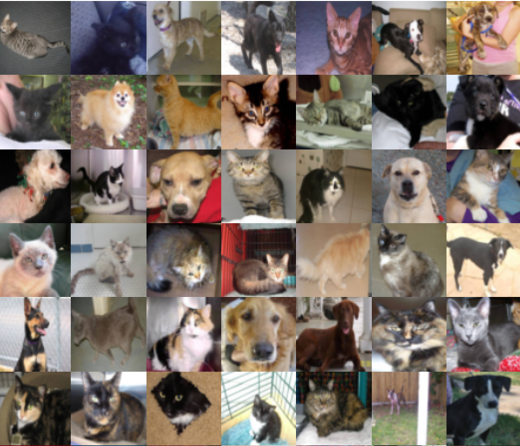
\includegraphics[scale=0.8]{res/catsdogs.png}
\caption[Caption for LOF]{Przykładowe zdjęcia z bazy danych serwisu Kaggle dla konkursu ,,Dogs vs. Cats'' \label{catsdogs}}
\end{figure} 

\subsubsection{Stworzone rozwiązanie}
System stworzony w~przypadku tego eksperymentu składał się z~dwóch głównych komponentów. W~celu wyodrębnienia wczytywania oraz~generowania danych stworzony został komponent nazwany DataProvider, który~pozwalał w~zręczny sposób podawać dane do~sieci. Drugim komponentem była sama sieć neuronowa. Ze~względy jednak na~duże wymogi obliczeniowe w~przypadku uczenia, możliwości dobrania odpowiedniej architektury oraz~optymalizowania parametrów były dość ograniczone. Wszystkie wykorzystywane obrazy zostały zmniejszony do~rozmiarów 64x64. Ostatecznie dobrana architektura sieci zawierała trzy warstwy konwolucyjne, jedną warstwę typu \textit{max pooling}, jedną warstwę w~pełni połączoną  oraz~jedną warstwę wyjściową. Warstwa wyjściowa składała się z~dwóch neuronów odpowiednio dla dwóch rozpoznawanych klas. W~przypadku warstw konwolucyjnych, wszystkie posiadały po~64 filtry z~tym, że~w~pierwszych dwóch stosowana była maska o~rozmiarach 7x7, a~w trzeciej 5x5.  Warstwa w~pełni połączona zawierała 512 neuronów. Obrazy generowane były dynamicznie podczas działania programu. Zastosowane zostały następujące operacje:
\begin{itemize}
\item rotacja obrazu w zakresie od 0 do 40 stopni,
\item przesunięcie w poziomie o długość do 20\% szerokości obrazu,
\item przesunięcie w pionie o długość do 20\% wysokości obrazu,
\item odbicie lustrzane obrazu w poziomie,
\item przybliżenie obrazu do 20\%.
\end{itemize}
Na rysunku \ref{catdogsimages} został przedstawiony obraz oryginalny oraz cztery obrazy wygenerowane na jego podstawie zgodnie z powyższymi parametrami.

\begin{figure}[ht!]
\centering
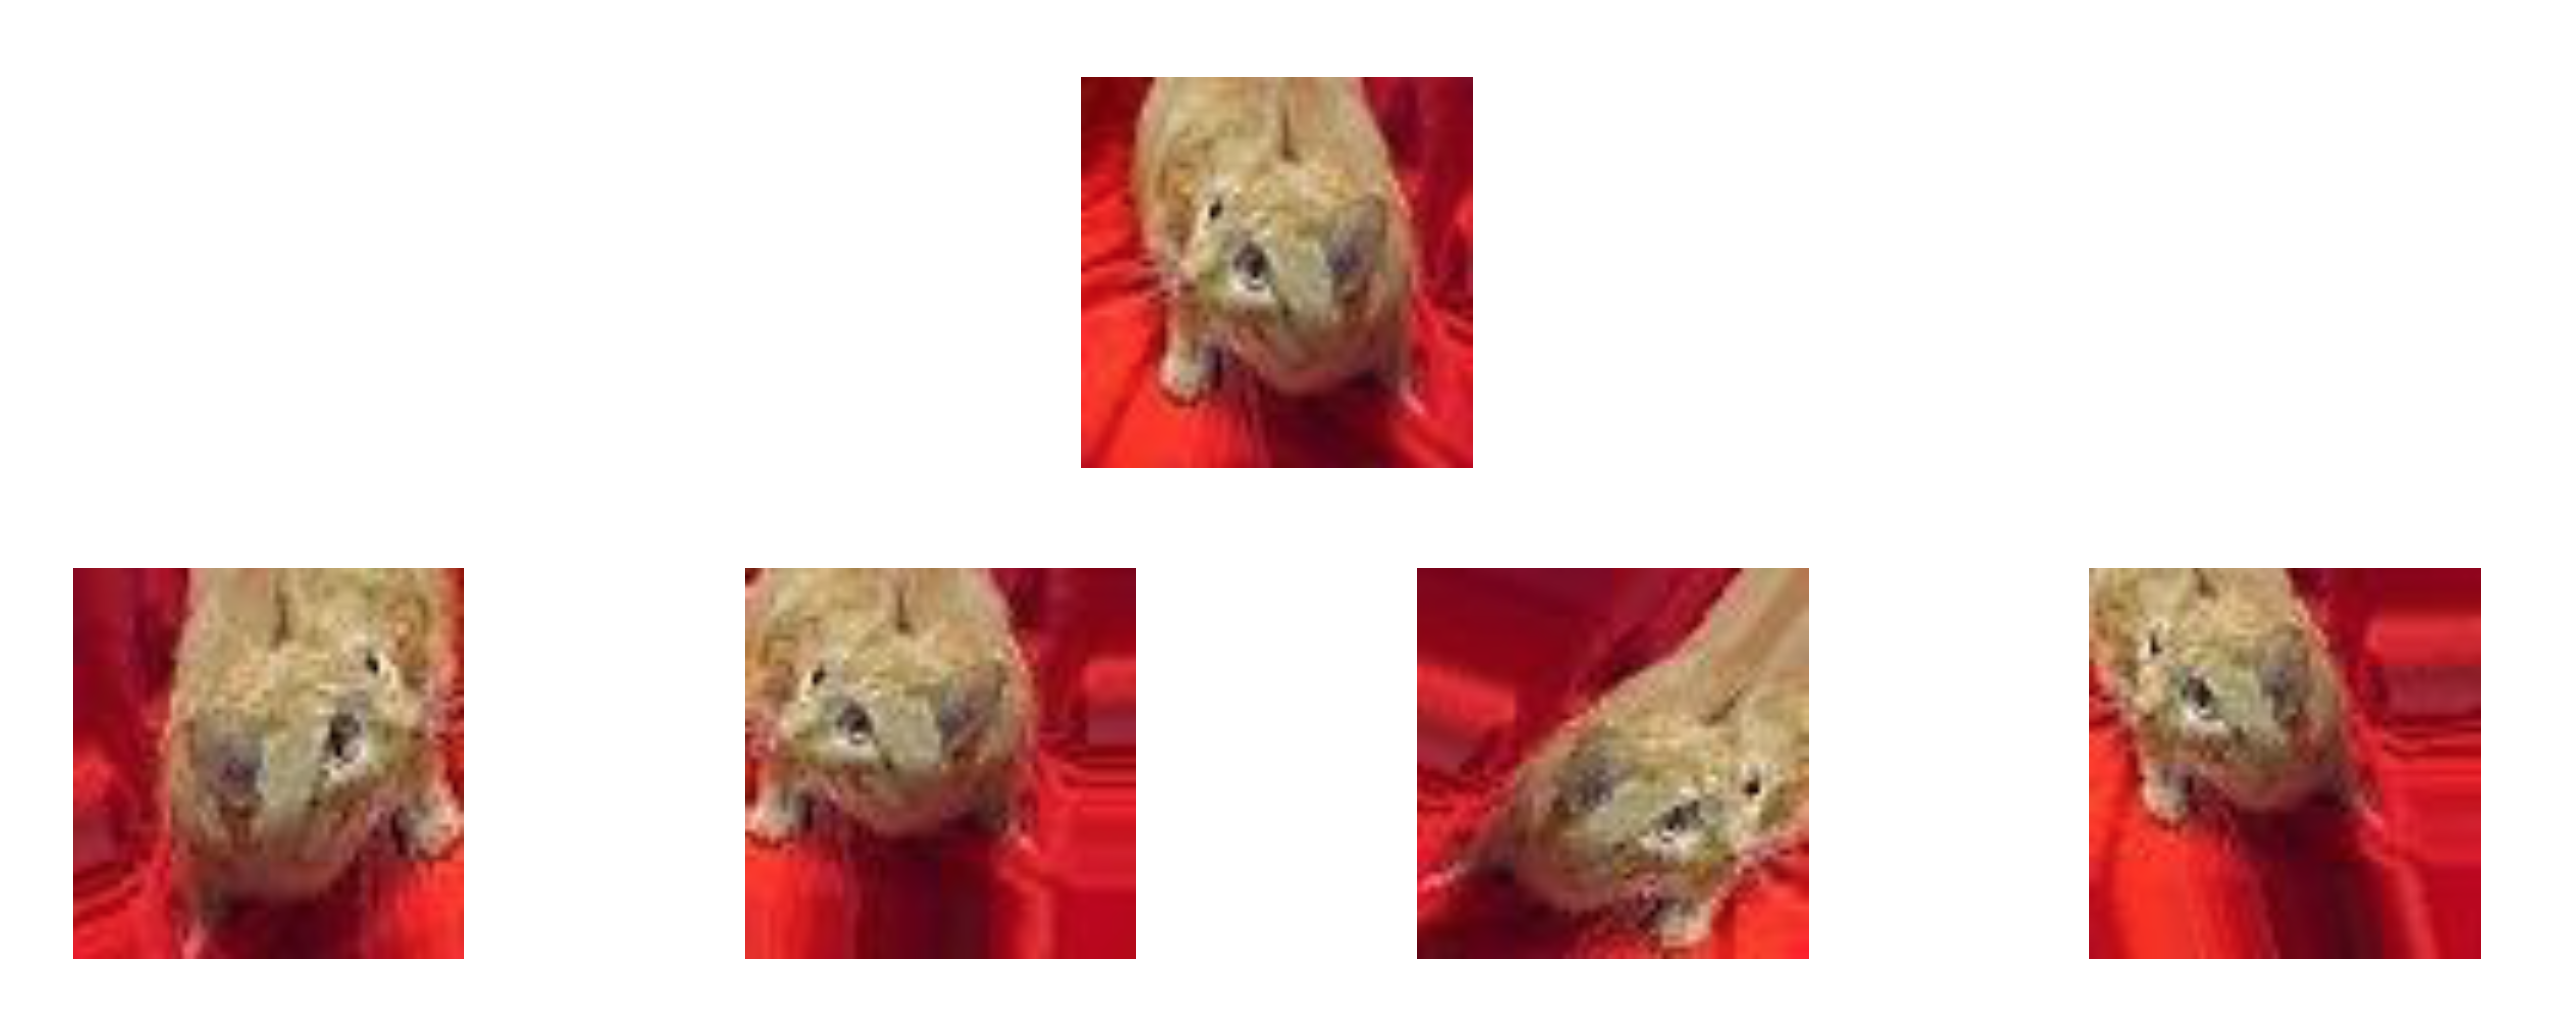
\includegraphics[scale=0.4]{res/catdogsaug.png}
\caption[Caption for LOF]{Obraz oryginalny oraz cztery obrazy wygenerowane na jego podstawie \label{catdogsimages}}
\end{figure} 

\subsubsection{Wyniki}
W~tabeli \ref{table:catdogs} przedstawione zostały wyniki dla sieci uruchamianej przy wykorzystaniu sztucznego powielania cech oraz~bez użycia tej techniki. Czy~powinienem tutaj jeszcze dodac jakies wyniki? Można przedstawić tutaj wykresy pokazujące skuteczność w~zależności od~iteracji dla obu przypadków, ale~wydaje mi się, że~nic to nie wnosi.

\begin{table}
\centering
\begin{tabular}{|c|c|}
\hline
Skuteczność uzyskana przy wykorzystaniu sztucznego powielania danych & $72\% \pm 2\%$ \\
\hline 
Skuteczność uzyskana bez wykorzystania sztucznego powielania danych & $69\% \pm 2\%$ \\
\hline 
 \end{tabular}
 \caption{Porównanie wyników z~zastosowaniem metody sztucznego powielania danych} \label{table:catdogs}
\end{table}

\subsubsection{Wnioski}
Sztuczne powiększanie zbioru danych, w analizowanym przypadku nie przyniosło spektakularnej poprawy. Jest to jednak wciąż 2~\%, które nie kosztuje zbyt wiele. Należy zwrócić uwagę też na to, iż w rzeczywistym przypadku operacja ta może przynieść więcej korzyści pod warunkiem odpowiedniego doboru jej parametrów, co nie zostało przeprowadzone w tym przypadku ze względu na ograniczone zasoby. 
\subsection{Walidacja krzyżowa}\label{cvChapter}
\subsubsection{Opis problemu}
W~tym podrozdziale autor starał się porównać system uczenia maszynowego działający przy zastosowaniu walidacji krzyżowej oraz~tradycyjnego podejścia w którym zbiór danych jest dzielony na~zbiór uczący, testowy oraz~walidacyjny. Przeprowadzona została kolejno optymalizacja parametrów dla czterech algorytmów tj. maszyna wektorów nośnych, sztuczne sieci neuronowe, las drzew decyzyjnych oraz~pojedyncze drzewo decyzyjne. W~każdym przypadku optymalizacja parametrów modelu została przeprowadzona za~pomocą metody walidacji krzyżowej oraz~wg tradycyjnego podejścia.  Algorytmy były testowane na~sztucznie wygenerowanych zbiorze zawierającym 7 atrybutów oraz~liczbę rekordów zawierającą się w zbiorze$ \{200, 500, 1000, 1500, 2000\}.$ Następnie porównane zostały wyniki dla parametrów wyznaczonych wg obu metod dla wszystkich testowanych algorytmów. Należy zwrócić tutaj szczególną uwagę na fakt, że optymalizacja przy pomocy walidacji krzyżowej odbywa się na poziomie doboru odpowiednich parametrów modelu. Po określeniu parametrów modelu, bez względu na metodę, którą do tego wykorzystaliśmy, następuje uczenie oraz walidacja finalnego modelu. W przypadku obu podejść, przy uczeniu oraz walidacji docelowego modelu, użyta zostaje dokładnie taka sama ilość danych. Porównanie użytej ilości danych w obu przypadkach zostało przedstawione na rysunku \ref{cvdata}. W przypadku tradycyjnego podejścia zbiór danych został podzielony na zbiór uczący stanowiący 60\% wszystkich danych, zbiór testowy stanowiący 20\% wszystkich danych oraz zbiór walidujący - również 20\% wszystkich danych. W przypadku walidacji krzyżowej, występowały tylko dwa zbiory tj. zbiór uczący oraz zbiór walidujący stanowiące kolejno 80\% oraz 20\% wszystkich danych. W celu uzyskania statystyki, obliczenia dla każdej metody dla konkretnej liczby rekordów powtórzone zostały 10 razy.

\begin{figure}[ht!]
\centering
\includegraphics[scale=0.6]{res/cvdata.png}
\caption[Caption for LOF]{Wykorzystanie danych w zleżności od zastosowanej metody doboru parametrów modelu\label{cvdata}}
\end{figure} 

\subsubsection{Stworzone rozwiązanie}
System stworzony w celu porównania skuteczności modelu w zależności od użytej metody doboru parametrów modelu składał się komponentów takich jak Main, Optimizer, oraz Configuration. Pierwszy z nich odpowiedzialny był za rozpoczęcie wykonania całej procedury, uwzględniając także wygenerowanie odpowiednich danych. Komponenty nazwane Optimizer oraz Configuration były kolejno odpowiedzialne za optymalizację parametrów modelu wg wybranej metody oraz ogólnej konfiguracji programu, gdzie można wybrać liczbę uruchomień optymalizacji czy też liczbę rekordów dla których porównanie powinno zostać przeprowadzone. Ze względu na dużą liczbę uruchomień optymalizacji, co jest procesem, który wykonuje się całkiem długo (w zależności od wybranych parametrów trwa to od kilkudziesięciu minut to kilku godzin), dodatkowo w zależności od wybranej metody optymalizacji parametrów, obliczenia prowadzone są z wykorzystaniem wielowątkowości. Znacznie przyspiesza to cały proces, zwłaszcza biorąc pod uwagę, że maszyna na której jest on przeprowadzany posiada 12 wątków.
 
\subsubsection{Wyniki}
Wyniki dla poszczególnych metod zostały przedstawione na rysunkach \ref{cv_ann}, \ref{cv_svm}, \ref{cv_forest} oraz \ref{cv_tree}.

\newcommand{\cvsize}{1}


\begin{figure}
\centering
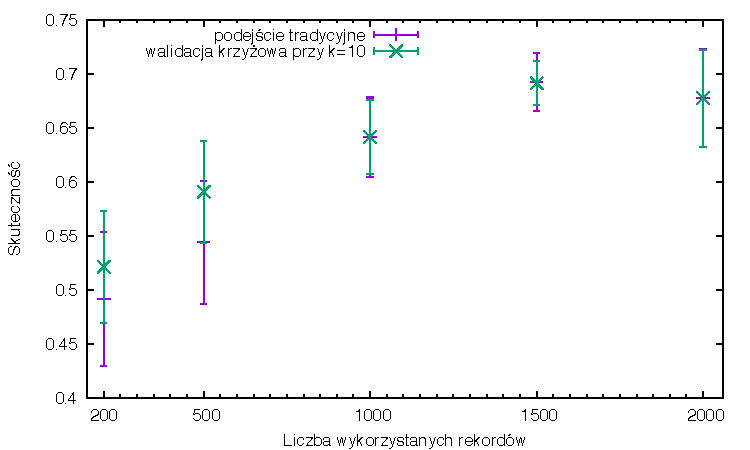
\includegraphics[scale=\cvsize]{res/cv_ann.pdf}
\caption[Caption for LOF]{Porównanie skuteczności modelu przy optymalizacji parametrów przy użyciu walidacji krzyżowej oraz tradycyjnego podejścia dla sztucznych sieci neuronowych\label{cv_ann}}
\end{figure}

\begin{figure}
\centering
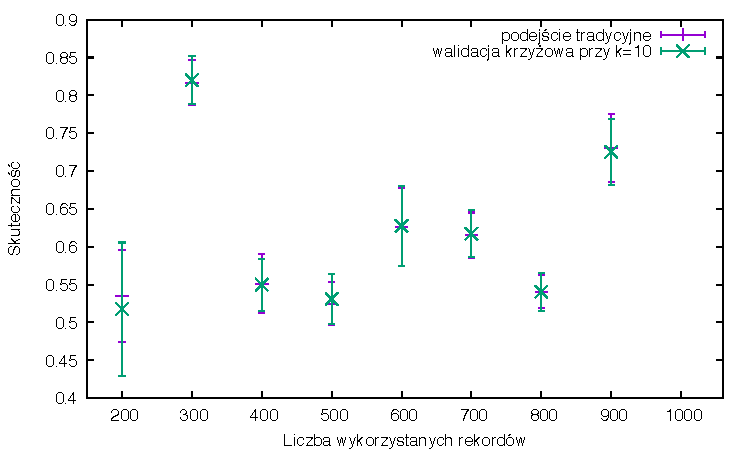
\includegraphics[scale=\cvsize]{res/cv_svm.pdf}
\caption[Caption for LOF]{Porównanie skuteczności modelu przy optymalizacji parametrów przy użyciu walidacji krzyżowej oraz tradycyjnego podejścia dla maszyny wektorów wspierających\label{cv_svm}}
\end{figure}

\begin{figure}
\centering
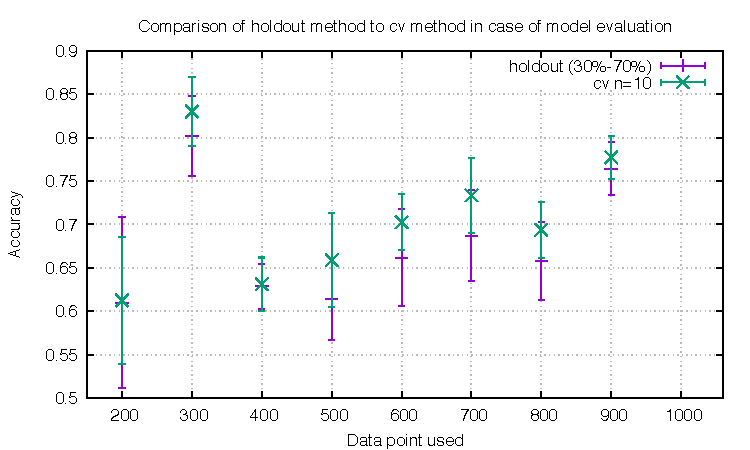
\includegraphics[scale=\cvsize]{res/cv_forest.pdf}
\caption[Caption for LOF]{Porównanie skuteczności modelu przy optymalizacji parametrów przy użyciu walidacji krzyżowej oraz tradycyjnego podejścia dla lasu drzew decyzyjnych\label{cv_forest}}
\end{figure}

\begin{figure}
\centering
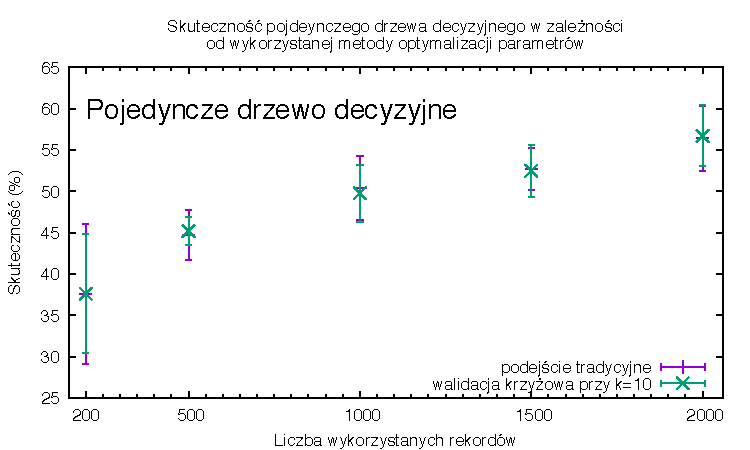
\includegraphics[scale=\cvsize]{res/cv_tree.pdf}
\caption[Caption for LOF]{Porównanie skuteczności modelu przy optymalizacji parametrów przy użyciu walidacji krzyżowej oraz tradycyjnego podejścia dla drzewa decyzyjnego\label{cv_tree}}
\end{figure}
  


\subsubsection{Wnioski}

\subsection{Ekstrakcja cech przy użyciu metod matematycznych}

\subsubsection{Opis problemu}
Matematycznymi metodami wykorzystanymi do~ekstrakcji cech danych były analiza głównych składowych oraz~liniowa analiza dyskryminacyjna. Przetestowane zostały cztery algorytmy uczenia maszynowego tj. maszyna wektorów nośnych, sztuczne sieci neuronowe, las drzew decyzyjnych oraz~pojedyncze drzewo decyzyjne. Wykorzystanym zbiorem danych był zbiór o~nazwie \textit{digits} dostępny w~bibliotece Scikit-Learn\footnote{\url{http://scikit-learn.org/stable/auto_examples/datasets/plot_digits_last_image.html}}. Posiada on 64 atrybuty odpowiadające poszczególnym pikselom na obrazie o rozmiarach 8x8. Każdy rekord zbioru reprezentuje jeden obraz przedstawiający jedną cyfrę. Cały zbiór podzielony jest na 10 klas odpowiadających kolejnym cyfrom. Eksperyment polegał na kolejno:
\begin{enumerate}
\item przeprowadzeniu optymalizacji parametrów modeli dla poszczególnych metod,
\item uczeniu oraz testowaniu systemu,
\end{enumerate}
w zależności od liczby rekordów oraz liczby atrybutów zbioru. Liczba rekordów dla których przeprowadzone zostały testy wynosiła 300 oraz~600. Obliczenia przeprowadzone zostały dla liczby atrybutów początkowo wynoszącej 64, która kolejno była zmniejszana wykorzystując PCA oraz LDA, aż do momentu gdy wynosiła 1. Celem było określenie czy, oraz na ile, ekstrakcja cech może pomóc w otrzymaniu wyższej skuteczności przy uczeniu maszynowym. Wszystkie obliczenia wykonane zostały w każdym przypadku 5 razy w celu uzyskania statystyki.

\subsubsection{Stworzone rozwiązanie}
Stworzony system składał się z komponentów takich jak Main, Optimizer oraz Configuration. Podobnie jak w eksperymencie opisanym w podrozdziale \ref{cvChapter} były odpowiedzialne kolejno za zadania uruchomienia głównego programu, optymalizacji parametrów modelu oraz konfigurację. Dodatkowo, w komponencie Main, znajduję się logika programu odpowiedzialna za redukcję wymiarowości zbioru danych. Także i w tym przypadku wykonywanie całej procedury dla różnych przypadków trwało dość długo tj. od kilku do kilkunastu godzin. 

\subsubsection{Wyniki}
Wyniki dla obliczeń przeprowadzonych dla liczby rekordów wynoszącej 300 zostały na rysunku \ref{fe_300}, natomiast dla liczby rekordów wynoszącej 600 na rysunku \ref{fe_600}.

\definecolor{Gray}{gray}{0.8}
\definecolor{White}{gray}{1}

\begin{table}
\centering
\begin{tabular}{|c|c|c|c|c|}
\hline
Skuteczność & Liczba cech & Liczba rekordów & metoda ekstrakcji & algorytm \\
\hline
\rowcolor{Gray}
$8.7 \% \pm 0.9 \%$ & $3$ & $ 300 $ & PCA & ann \\
\hline
\rowcolor{Gray}
$2.1 \% \pm 0.2 \%$ & $64$ & $ 300 $ & PCA & ann \\
\hline
\rowcolor{White}
$9.0 \% $ & $3$ & $ 300 $ & PCA & svm \\
\hline
\rowcolor{White}
$2.0 \% $ & $64$ & $ 300 $ & PCA & svm \\
\hline
\rowcolor{Gray}
$10.6 \% \pm 0.4 \%$ & $3$ & $ 300 $ & PCA & forest \\
\hline
\rowcolor{Gray}
$3.3 \% \pm 0.2 \%$ & $64$ & $ 300 $ & PCA & forest \\
\hline
\rowcolor{White}
$11.4 \% \pm 0.2 \%$ & $3$ & $ 300 $ & PCA & tree \\
\hline
\rowcolor{White}
$5.2 \% \pm 0.2 \%$ & $64$ & $ 300 $ & PCA & tree \\
\hline
\rowcolor{Gray}
$28.5 \% \pm 2.3 \%$ & $1$ & $ 300 $ & LDA & ann \\
\hline
\rowcolor{Gray}
$21.3 \% \pm 0.4 \%$ & $64$ & $ 300 $ & LDA & ann \\
\hline
\rowcolor{White}
$27.0 \% $ & $4$ & $ 300 $ & LDA & svm \\
\hline
\rowcolor{White}
$20.0 \% $ & $64$ & $ 300 $ & LDA & svm \\
\hline
\rowcolor{Gray}
$30.8 \% \pm 1.4 \%$ & $1$ & $ 300 $ & LDA & forest \\
\hline
\rowcolor{Gray}
$20.5 \% \pm 4.3 \%$ & $64$ & $ 300 $ & LDA & forest \\
\hline
\rowcolor{White}
$31.5 \% \pm 0.4 \%$ & $1$ & $ 300 $ & LDA & tree \\
\hline
\rowcolor{White}
$17.9 \% \pm 1.1 \%$ & $64$ & $ 300 $ & LDA & tree \\
\hline
\rowcolor{Gray}
$72.2 \% \pm 3.3 \%$ & $5$ & $ 600 $ & PCA & ann \\
\hline
\rowcolor{Gray}
$46.2 \% \pm 1.4 \%$ & $64$ & $ 600 $ & PCA & ann \\
\hline
\rowcolor{White}
$68.5 \%$ & $5$ & $ 600 $ & PCA & svm \\
\hline
\rowcolor{White}
$50.0\%$ & $64$ & $ 600 $ & PCA & svm \\
\hline
\rowcolor{Gray}
$64.4 \%\pm 1.8\%$ & $5$ & $ 600 $ & PCA & forest \\
\hline
\rowcolor{Gray}
$40.1 \%\pm 5.7\%$ & $64$ & $ 600 $ & PCA & forest \\
\hline
\rowcolor{White}
$64.4 \%\pm 1.7\%$ & $5$ & $ 600 $ & PCA & tree \\
\hline
\rowcolor{White}
$51.9 \% \pm 2.8 \%$ & $64$ & $ 600 $ & PCA & tree \\
\hline
\rowcolor{Gray}
$73.0\%\pm 1.0\%$ & $3$ & $ 600 $ & LDA & ann \\
\hline
\rowcolor{Gray}
$27.5 \%\pm 1.3\%$ & $64$ & $ 600 $ & LDA & ann \\
\hline
\rowcolor{White}
$74.0\%$ & $3$ & $ 600 $ & LDA & svm \\
\hline
\rowcolor{White}
$27.0\%$ & $64$ & $ 600 $ & LDA & svm \\
\hline
\rowcolor{Gray}
$70.4 \%\pm 2.3\%$ & $3$ & $ 600 $ & LDA & forest \\
\hline
\rowcolor{Gray}
$26.4 \%\pm 6.2\%$ & $64$ & $ 600 $ & LDA & forest \\
\hline
\rowcolor{White}
$72.1 \%\pm 1.1\%$ & $3$ & $ 600 $ & LDA & tree \\
\hline
\rowcolor{White}
$34.7 \%\pm 5.3\%$ & $64$ & $ 600 $ & LDA & tree \\
\hline

 \end{tabular}
 \caption{Najlepsze uzyskane wyniki modeli uczonych przy wykorzystaniu zbioru danych po redukcji cech w porównaniu do modeli uczonych przed wykorzystaniem ekstrakcji cech} \label{table:featureExtraction}
\end{table}


\begin{table}[]
\centering

\begin{tabular}{llllll}
                                                         &                                                              & \multicolumn{2}{c}{}                                                                                                                                    &  &  \\ \cline{3-4}
                                                         & \multicolumn{1}{l|}{}                                        & \multicolumn{1}{l|}{\cellcolor[HTML]{9B9B9B}{\color[HTML]{000000} PCA}} & \multicolumn{1}{l|}{\cellcolor[HTML]{9B9B9B}{\color[HTML]{000000} LDA}} &  &  \\ \cline{2-4}
\multicolumn{1}{c|}{}                                    & \multicolumn{1}{l|}{\cellcolor[HTML]{9B9B9B}300 rekordów} & \multicolumn{1}{l|}{$7.27 \%$}                                           & \multicolumn{1}{l|}{$9.53\%$}                                            &  &  \\ \cline{2-4}
\multicolumn{1}{c|}{\multirow{-2}{*}{}} & \multicolumn{1}{l|}{\cellcolor[HTML]{9B9B9B}600 rekordów} & \multicolumn{1}{l|}{$20.32 \%$}                                            & \multicolumn{1}{l|}{$43.47\%$}                                           &  &  \\ \cline{2-4}
                                                         &                                                              &                                                                                     &                                                                                     &  & 
\end{tabular}
\caption{Średnia poprawa skuteczności klasyfikacji w zależności od liczby danych oraz metody ekstrakcji} \label{table:confusionmatrix}
\end{table}


\newcommand{\fesize}{0.45}

\begin{figure}
\centering
\begin{minipage}{.5\textwidth}

\centering
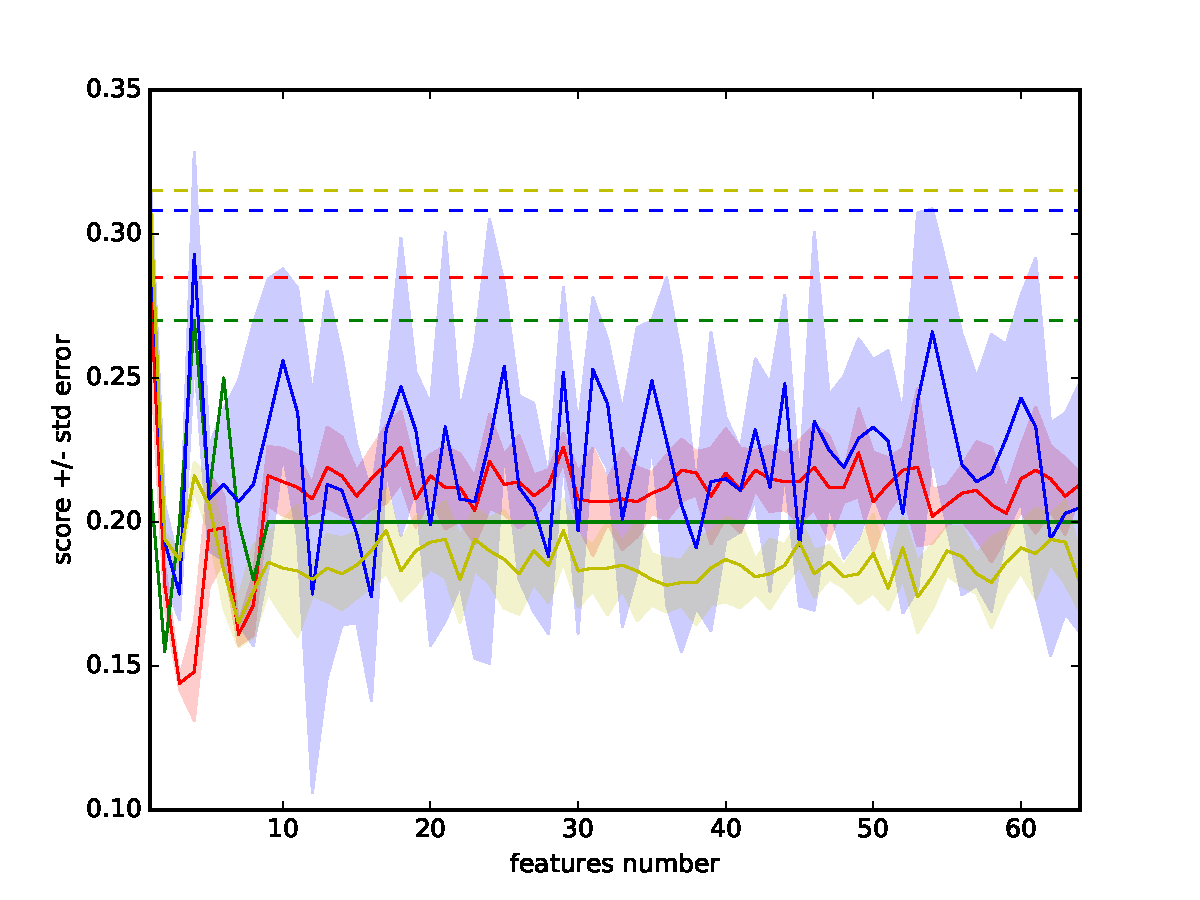
\includegraphics[scale=\fesize]{res/digits_300_all_LinearDiscriminantAnalysis.pdf}

  
\end{minipage}%
\begin{minipage}{.5\textwidth}

\centering
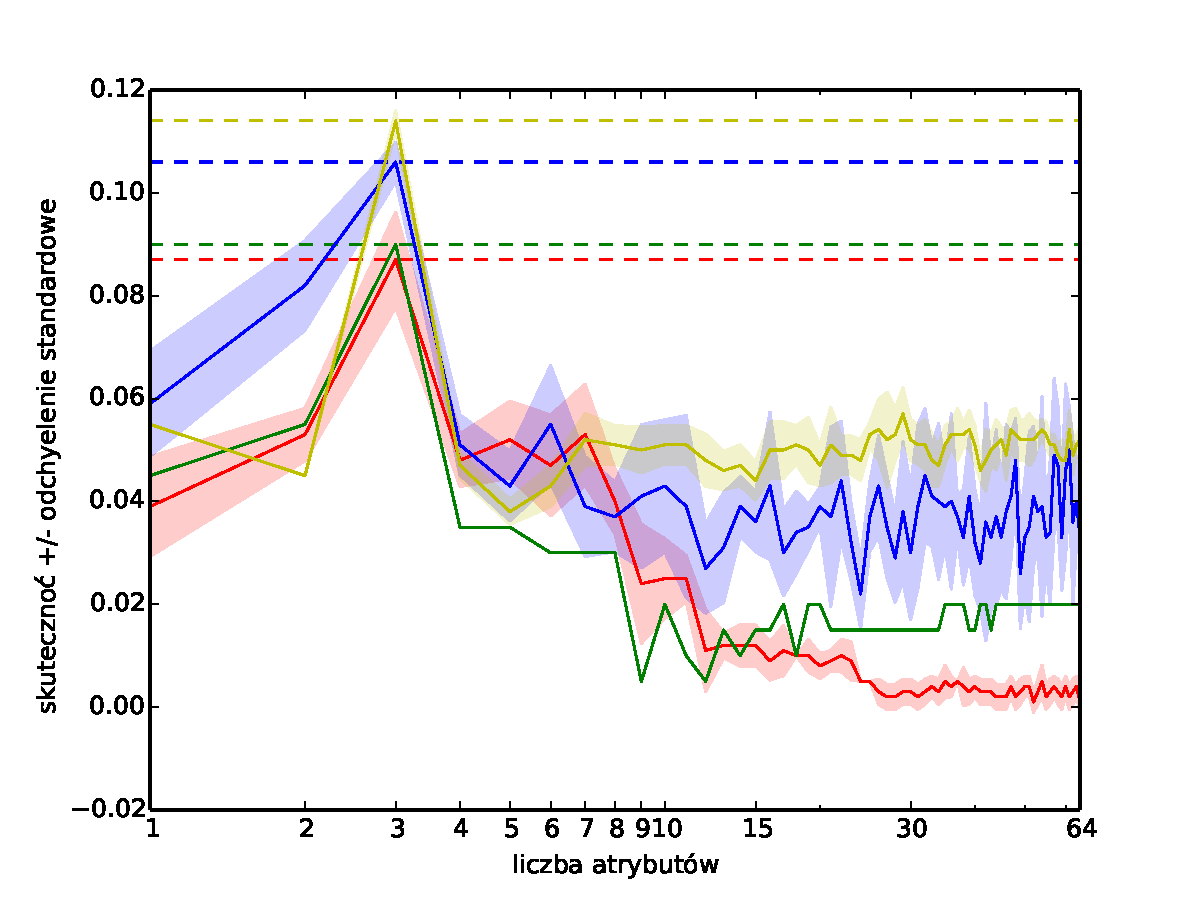
\includegraphics[scale=\fesize]{res/digits_300_all_PCA.pdf}
  
\end{minipage}
\caption[Caption for LOF]{Zależność skuteczności od liczby wykorzystanych atrybutów przy użyciu 300 rekordów do stworzenia systemu\label{fe_300}}
\end{figure}

\begin{figure}
\centering
\begin{minipage}{.5\textwidth}

\centering
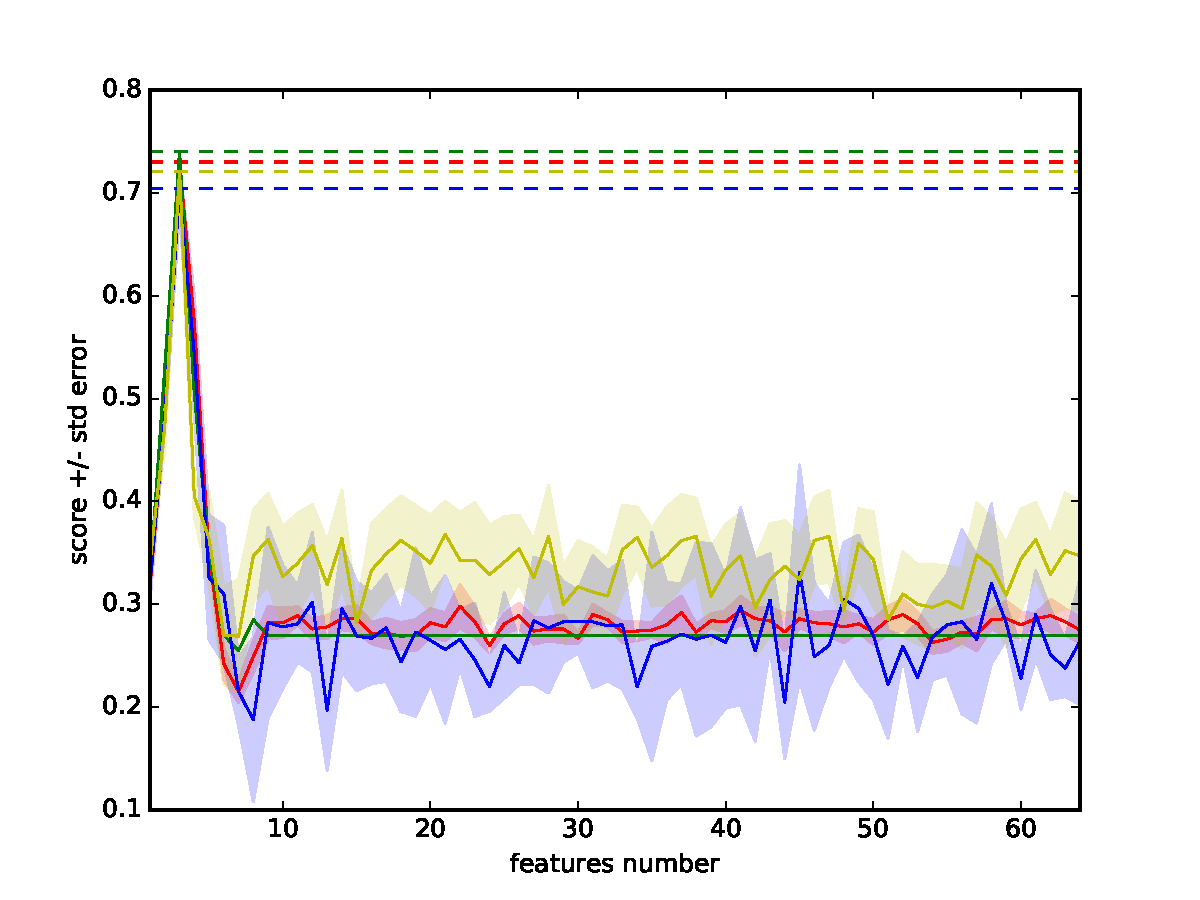
\includegraphics[scale=\fesize]{res/digits_600_all_LinearDiscriminantAnalysis.pdf}

  
\end{minipage}%
\begin{minipage}{.5\textwidth}

\centering
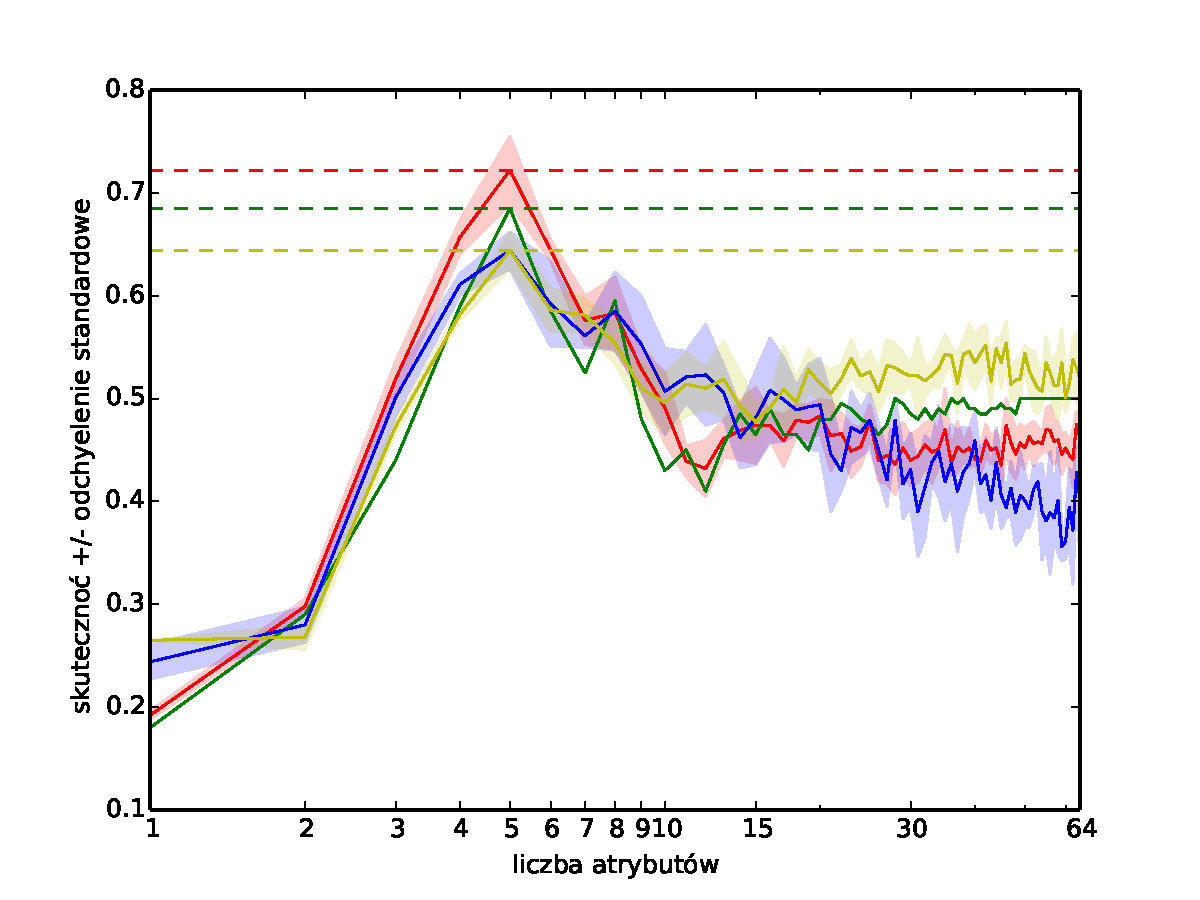
\includegraphics[scale=\fesize]{res/digits_600_all_PCA.pdf}
  
\end{minipage}
\caption[Caption for LOF]{Zależność skuteczności od liczby wykorzystanych atrybutów przy użyciu 600 rekordów do stworzenia systemu\label{fe_600}}
\end{figure}



\subsubsection{Wnioski}

\subsection{Ekstrakcja cech przy użyciu ,,wiedzy''}
\subsubsection{Opis problemu}
W~niniejszym podrozdziale rozważanym zagadnieniem była ekstrakcja cech przy użyciu ,,wiedzy'', która polegaa na transformacji danych do~przestrzeni o~mniejszej wymiarowości przy wykorzystaniu wiedzy, którą posiadamy na~temat naszych danych. Pomysł na~ten eksperyment został zaczerpnięty z~pracy~\cite{higgs1}. Wykorzystane zostały także dane opisane w~artykule, które~są danymi zebranymi z~detektorów cząstek ulokowanych w~Wielkim Zderzaczu Hadronów (\textit{Large Hadron Collider}, LHC) będącym największym na~świecie akceleratorem cząstek, który~ulokowany jest w~Europejskim Ośrodku Badań Jądrowych CERN w~pobliżu Genewy. Głównym celem działania LHC jest zgłębienie wiedzy na~temat cząstek elementarnych. W~celu izolacji sygnału od~tła w~przypadku posiadania danych z~odpowiednich detektorów szeroko wykorzystywane jest uczenie maszynowe. Artykuł opisuje wykorzystanie głębokich sieci neuronowych dla problemu wyodrębnienia cząstki Higgsa. Udostępnione dane zawierają 11 milionów rekordów dla których określonych jest 21 cech fizycznych tzw. niskiego poziomu. Każdy rekord opisany jest także za~pomocą 7 atrybutów wysokiego poziomu, które~obliczone zostały na~podstawie cech niskiego poziomu. Celem obliczeń było pokazanie, że~poniżej pewnej ilości danych, użycie niskiego poziomu daje gorsze wyniki niż wykorzystanie cech wysokiego poziomu. Obok głębokiej sieci neuronowej, wykorzystane zostały algorytmy takiej jak~tradycyjne sieć neuronowa, las drzew decyzyjnych oraz~pojedyncze drzewo decyzyjne. Dla wszystkich wymienionych tradycyjnych algorytmów uczenia maszynowego przeprowadzona została optymalizacja parametrów. W~przypadku głębokiej sieci neuronowej nie miało to nie miejsca ze~względu na~bardzo długi czas uczenia. W przypadku wszystkich metod obliczenia przeprowadzone zostały dla cech wysokiego oraz niskiego poziomu, a także dla różnej ilości danych, które~były fragmentami całego udostępnionego zbioru. Rozważone zostały ułamki $a$ całego zbioru przy czym $a\in\{0,001; 0,005; 0,01; 0,05; 0,1; 0,2; 0,3; 0,4; 0,5\}$. 

\subsubsection{Stworzone rozwiązanie}
Stworzony system składał się z trzech elementów z których można wyróżnić: HiggsModel, Optimizer oraz Configuration. Były odpowiedzialne kolejno za tworzenie głębokie sieci neuronowej (oparty na pracy \cite{higgs2}), optymalizację parametrów dla poszczególnych algorytmów oraz konfiguracji programu. W przypadku głębokiej sieci neuronowej, wykorzystana została sieć posiadająca 6 warstw ukrytych po~500 neuronów w~każdej. 


\subsubsection{Wyniki}
Na rysunkach \ref{higgsall1} oraz \ref{higgsall2} przedstawione została krzywa ROC dla $a\in\{0.001, 0.005, 0.01, 0.05, 0.1\}$ w pierwszym przypadku oraz dla $a\in\{0.2, 0.3, 0.4, 0.5\}$ w drugim przypadku. Porównanie AUC ROC zostało natomiast przedstawione na rysunku \ref{higgssummary}.

\begin{figure}[ht!]
\centering
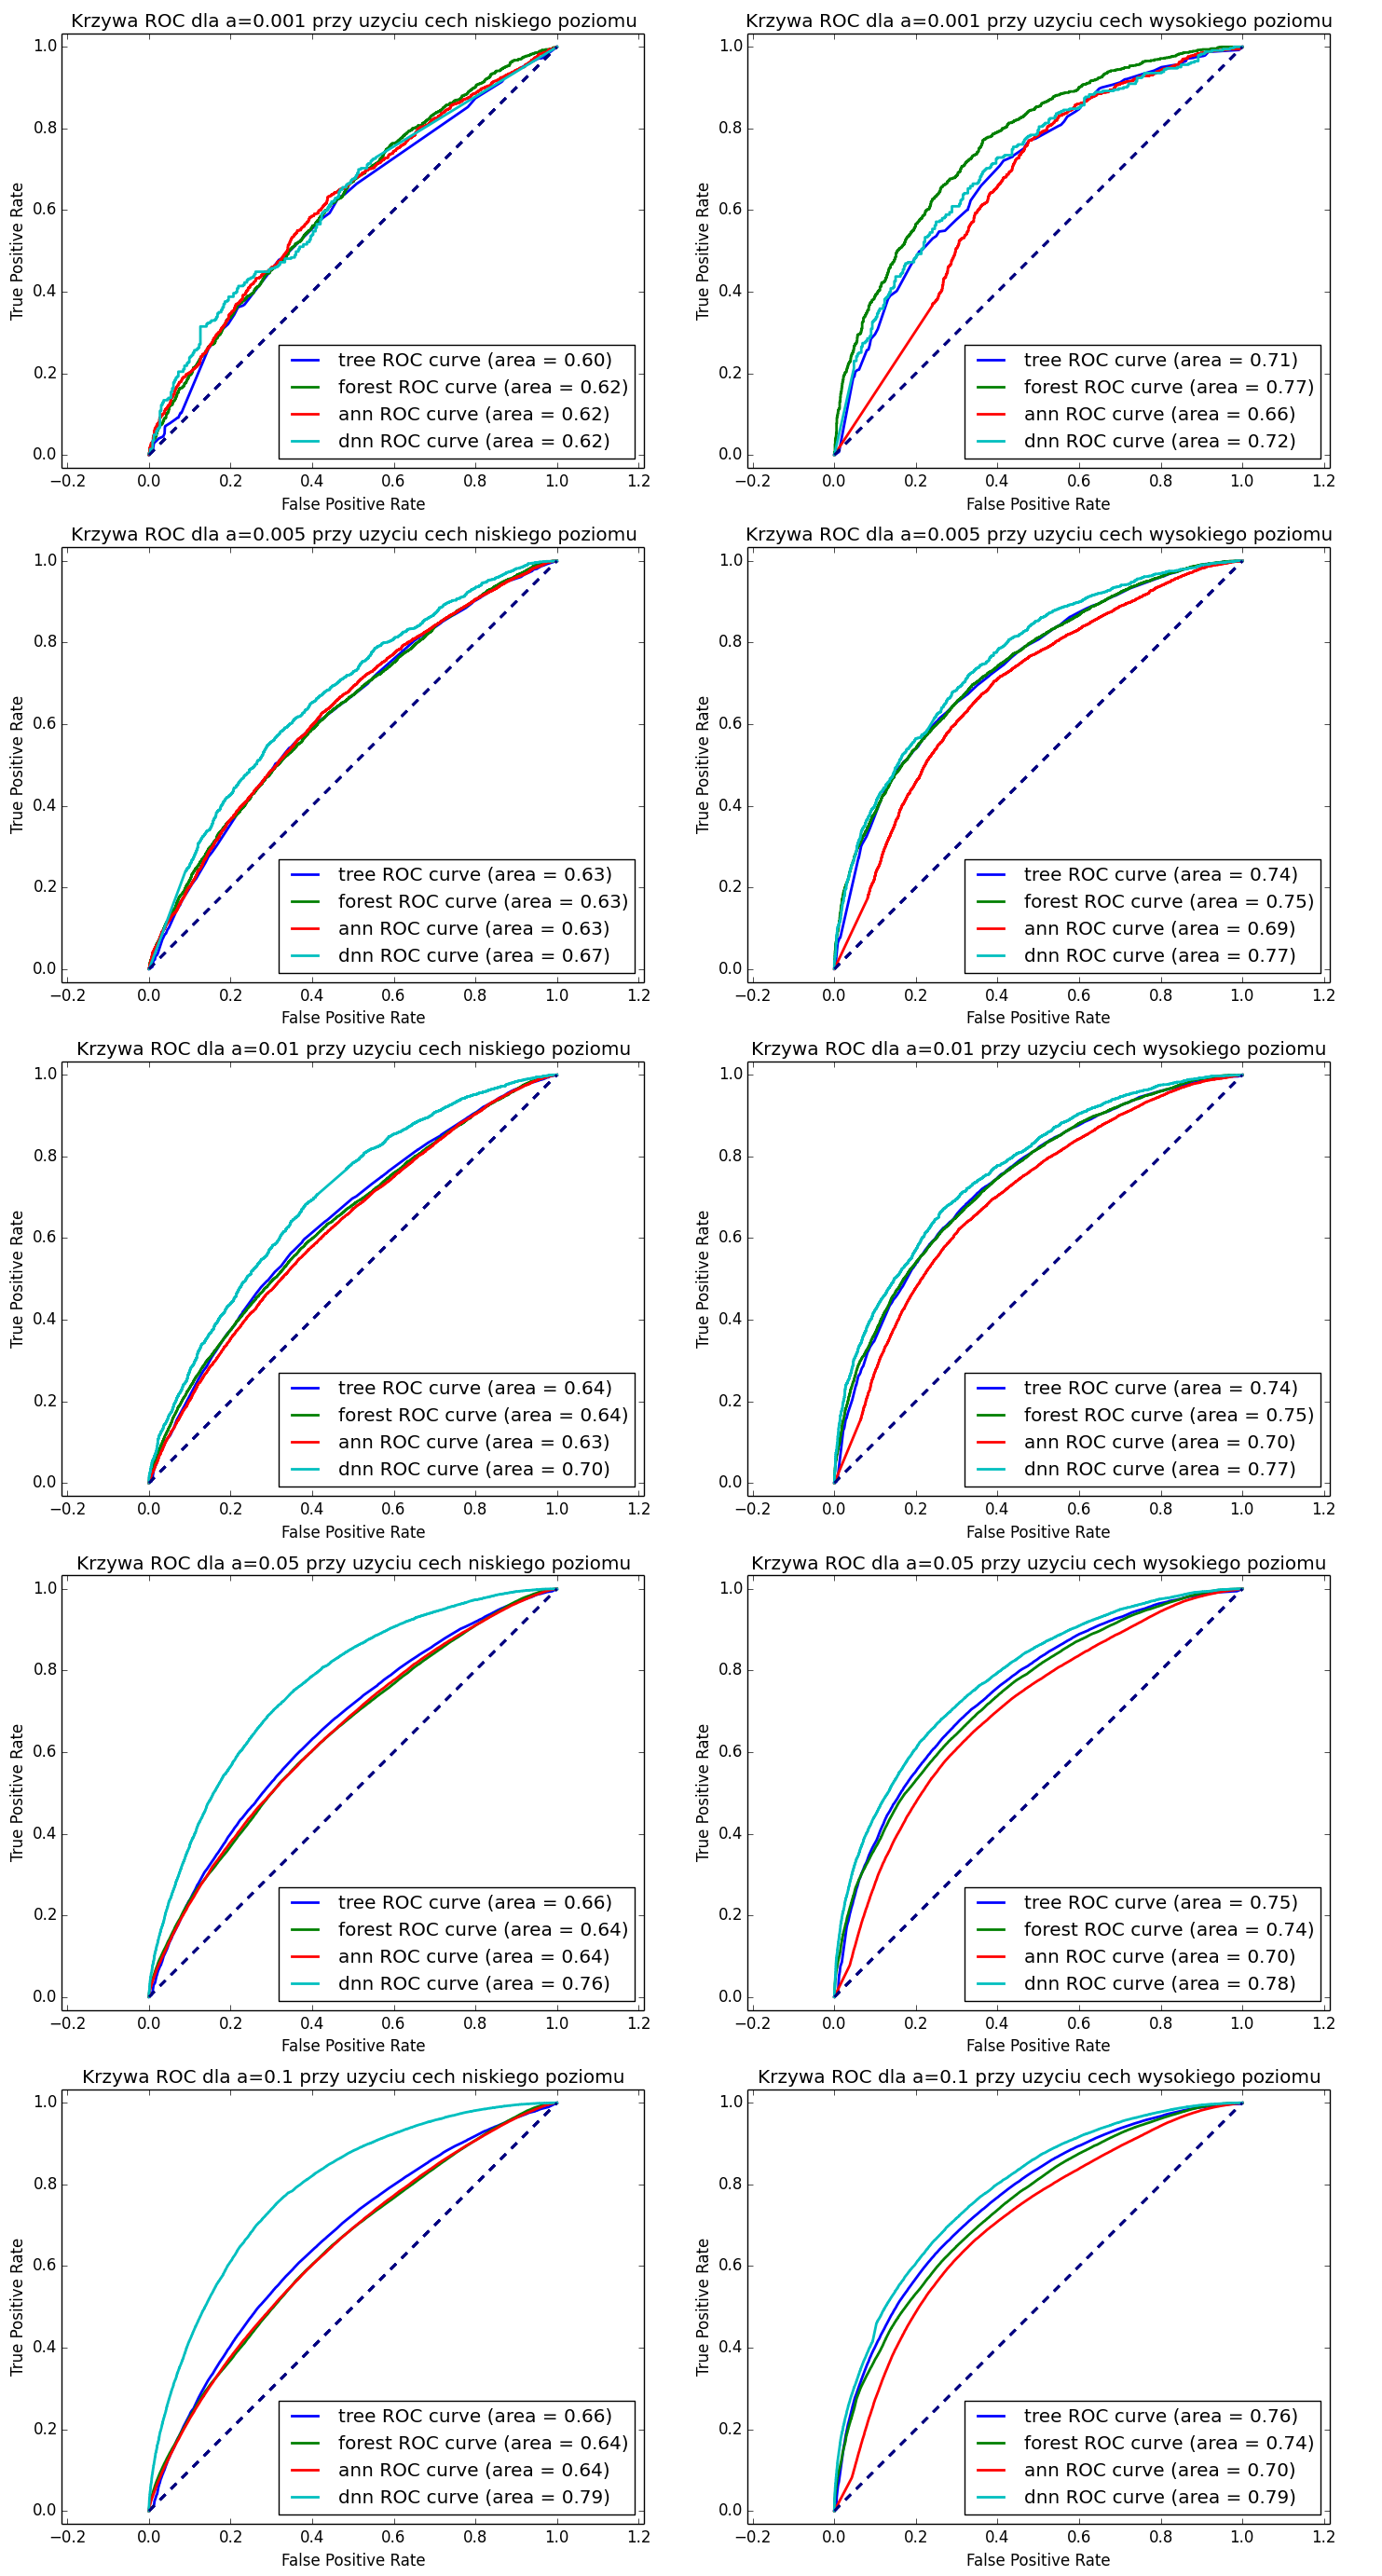
\includegraphics[scale=0.3]{res/all1.png}
\caption[Caption for LOF]{Krzywa ROC dla $a\in\{0.001, 0.005, 0.01, 0.05, 0.1\}$\label{higgsall1}}
\end{figure} 

\begin{figure}[ht!]
\centering
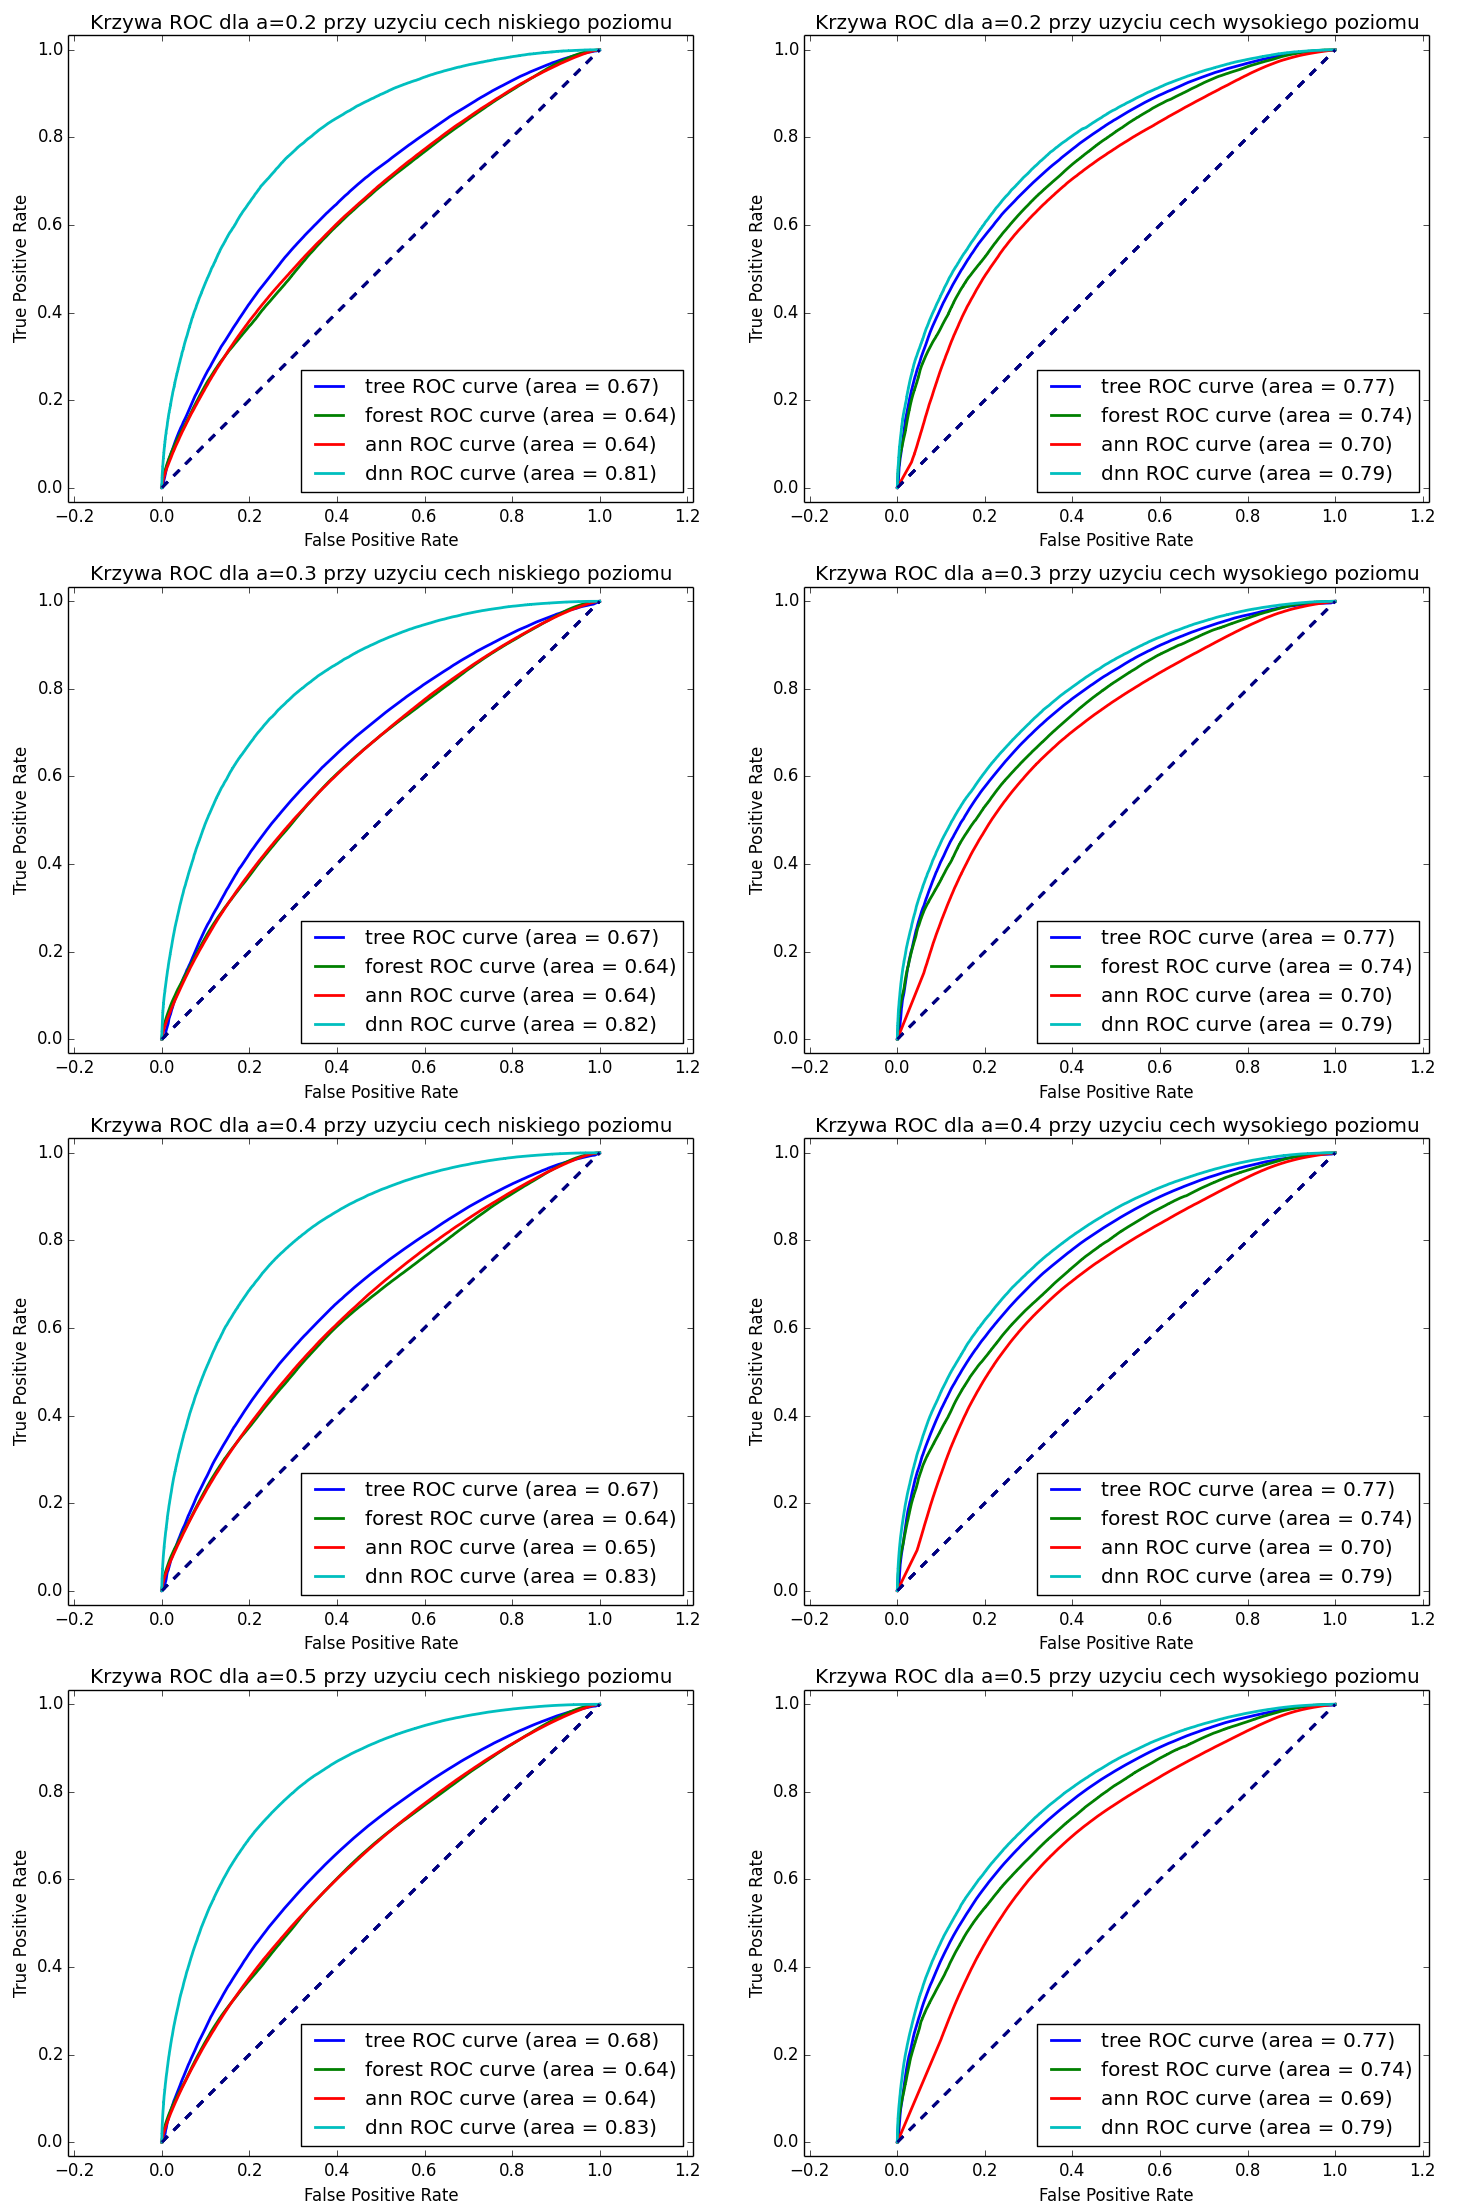
\includegraphics[scale=0.3]{res/all2.png}
\caption[Caption for LOF]{Krzywa ROC dla $a\in\{0.2, 0.3, 0.4, 0.5\}$\label{higgsall2}}
\end{figure} 

\begin{figure}[ht!]
\centering
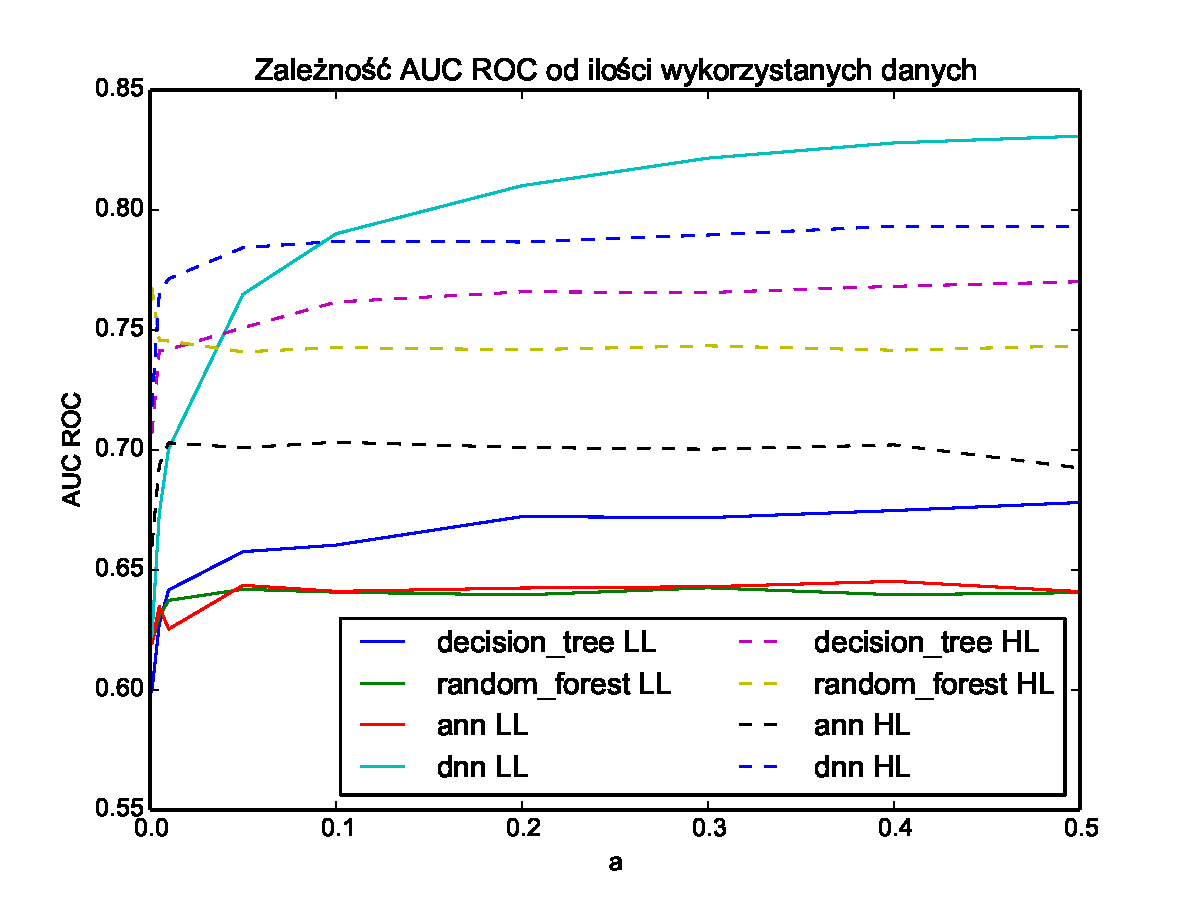
\includegraphics[scale=0.8]{res/higgssummary.pdf}
\caption[Caption for LOF]{Porównanie AUC ROC w zależności od rodzaju wykorzystanych cech dla wszystkich testowanych metod\label{higgssummary}}
\end{figure} 

\subsubsection{Wnioski}

